% !TeX program = xelatex
\ifdefined\BookMaster\else
\documentclass[11pt,oneside]{article}
% !TeX program = xelatex
\usepackage[b5paper,left=22mm,right=22mm,top=20mm,bottom=22mm,footskip=11mm]{geometry}
\usepackage{fontspec}
\setmainfont{TeX Gyre Termes}
\setsansfont{TeX Gyre Heros}
\usepackage{amsmath,amssymb,mathtools,amsthm}
\renewcommand{\cdots}{\mathinner{\cdotp\cdotp\cdotp}}
\usepackage{graphicx,adjustbox,array,booktabs,longtable,multirow,enumitem,changepage,needspace}
\usepackage[table]{xcolor}
\usepackage{fancyhdr}
\raggedbottom
\interfootnotelinepenalty=10000
\newcommand{\BookFootnote}[2]{\begingroup\renewcommand{\thefootnote}{\fnsymbol{footnote}}\footnote[#1]{#2}\endgroup}
\newcommand{\BookFootnoteMark}[1]{\begingroup\renewcommand{\thefootnote}{\fnsymbol{footnote}}\footnotemark[#1]\endgroup}
\newcommand{\BookFootnoteText}[2]{\begingroup\renewcommand{\thefootnote}{\fnsymbol{footnote}}\footnotetext[#1]{#2}\endgroup}
\newenvironment{BookFloat}[1]{\par\addvspace{.6\baselineskip}\noindent\def\BookFloatID{#1}\begin{minipage}{\linewidth}\phantomsection\label{bookfloat:#1:start}}{\phantomsection\label{bookfloat:\BookFloatID:end}\end{minipage}\par\addvspace{.6\baselineskip}}

\usepackage[unicode,hidelinks]{hyperref}
\pagestyle{fancy}
\fancyhf{}
\newcommand{\BookFooter}{}
\fancyfoot[L]{\parbox[b]{\dimexpr\textwidth-15mm}{\footnotesize\BookFooter}}
\fancyfoot[R]{\footnotesize\thepage}
\renewcommand{\headrulewidth}{0pt}
\renewcommand{\footrulewidth}{0pt}
\setlength{\parindent}{0pt}
\setlength{\parskip}{0.2em}
\setlength{\emergencystretch}{3em}
\setlist{nosep,leftmargin=1.7em,labelsep=.65em}
\newif\ifBookNarrative
\BookNarrativetrue
\newenvironment{BookBody}{\setlength{\parindent}{0pt}}{}
\newcommand{\BookStatement}[1]{\par\addvspace{.6\baselineskip}\noindent #1\enspace\ignorespaces}
\newcommand{\BookLabel}[1]{\par\addvspace{.6\baselineskip}\needspace{3\baselineskip}\noindent\textbf{#1}\quad\ignorespaces}
\newcommand{\BookHeading}[1]{\par\addvspace{\baselineskip}\needspace{4\baselineskip}\noindent{\large\bfseries #1}\par\medskip}
\newcommand{\BookSubheading}[1]{\par\addvspace{.7\baselineskip}\needspace{3\baselineskip}\noindent{\bfseries #1}\par\smallskip}
\newcommand{\BookTextHeading}[1]{\par\addvspace{.7\baselineskip}\needspace{3\baselineskip}\noindent #1\par\smallskip}
\newcommand{\BookSectionTitle}[2]{\par\addvspace{1.2\baselineskip}\needspace{5\baselineskip}\noindent\colorbox{gray!25}{\sffamily\bfseries\small SECTION #1}\quad{\large\bfseries #2}\par\medskip}
\newcommand{\BookExerciseTitle}[1]{\par\addvspace{\baselineskip}\needspace{4\baselineskip}\noindent{\color{gray}\rule{1.5mm}{1.5mm}}\enspace{\large\bfseries Exercises #1}\par\medskip}
\newcommand{\BookBullet}[1]{\begin{list}{\textbullet}{\setlength{\leftmargin}{1.7em}\setlength{\labelwidth}{1em}\setlength{\labelsep}{.7em}\setlength{\topsep}{0pt}\setlength{\parsep}{0pt}\setlength{\itemsep}{0pt}}\item #1\end{list}}
\newcommand{\BookExercise}[2]{\begin{list}{\textbf{#1}}{\setlength{\leftmargin}{2.2em}\setlength{\labelwidth}{1.5em}\setlength{\labelsep}{.7em}\setlength{\topsep}{.15em}\setlength{\parsep}{0pt}\setlength{\itemsep}{0pt}}\item #2\end{list}}
\newcommand{\BookEnd}[1]{\unskip\nobreak\hfill\ensuremath{#1}}
\newcommand{\BookSource}[2]{\phantomsection\label{sourcepage:#1}} % Source-page anchors, retained through reflow.
\usepackage{multicol}
\usepackage{tikz}
\newcommand{\BookPartEntry}[2]{\par\noindent\makebox[17mm][l]{\bfseries Section #1}#2\par}
\newcommand{\BookPartTitle}[3]{\par\bigskip\noindent\begin{tikzpicture}\node[anchor=north west,inner sep=0pt,outer sep=0pt] (bookpart) at (0,0) {\begin{minipage}{\dimexpr\linewidth-.5pt}\hspace*{26mm}\begin{minipage}[t]{\dimexpr\linewidth-26mm}\begin{adjustbox}{max width=\linewidth}{\fontsize{20}{24}\selectfont\bfseries #2}\end{adjustbox}\par\vspace{6mm}\hrule\vspace{6mm}{\sffamily\footnotesize\setlength{\parskip}{.3em}#3}\vspace{3mm}\end{minipage}\end{minipage}};\path[shade,top color=gray!60,bottom color=white] (0,0) rectangle ([xshift=24mm]bookpart.south west);\node[anchor=north,font=\sffamily\bfseries\small] at (12mm,-2mm) {PART};\node[anchor=north,font=\sffamily\bfseries\Huge] at (12mm,-7mm) {#1};\end{tikzpicture}\par\bigskip}
\newsavebox{\BookMathBox}
\makeatletter
\newcommand{\BookInline}[1]{\leavevmode\hskip0pt\relax\begingroup\in@{\begin}{#1}\ifin@\sbox{\BookMathBox}{\(#1\)}\ifdim\wd\BookMathBox>\dimexpr\linewidth-1em\relax\resizebox{\dimexpr\linewidth-1em\relax}{!}{\usebox{\BookMathBox}}\else\(#1\)\fi\else\in@{\left}{#1}\ifin@\sbox{\BookMathBox}{\(#1\)}\ifdim\wd\BookMathBox>\dimexpr\linewidth-1em\relax\resizebox{\dimexpr\linewidth-1em\relax}{!}{\usebox{\BookMathBox}}\else\(#1\)\fi\else\(#1\)\fi\fi\endgroup\hskip0pt\relax}
\makeatother
\DeclareMathOperator{\Aut}{Aut}
\DeclareMathOperator{\End}{End}
\DeclareMathOperator{\Hom}{Hom}
\DeclareMathOperator{\GF}{GF}
\DeclareMathOperator{\irr}{irr}
\DeclareMathOperator{\lt}{lt}
\DeclareMathOperator{\lp}{lp}
\providecommand{\textcircled}[1]{\textnormal{(#1)}}

\begin{document}
\fi
\renewcommand{\BookFooter}{Section 14 Group Action on a Set}
\pdfbookmark[0]{Section 14 Group Action on a Set}{14_group_action_on_a_set}
\ifdefined\BookMaster\else\setcounter{page}{132}\fi
% Source PDF page 149; original printed page 132
\BookSource{149}{132}
\BookNarrativetrue

\begin{BookBody}

\BookSectionTitle{14}{Group Action on a Set\label{bookfootnote:149:2:ref}\BookFootnote{2}{\label{bookfootnote:149:2:text}This section is a prerequisite only for Sections 15 and 17.}}

\noindent We have seen examples of how groups may\textit{ act on things}, like the group of symmetries of a triangle or of a square, the group of rotations of a cube, the general linear group acting on \BookInline{\mathbb{R}^{n},\allowbreak } and so on. In this section we give the general notion of group action and apply it to learn more about finite groups. The next section will give applications to counting.

\BookTextHeading{\textbf{The Notion of a Group Action}  }

\noindent Definition 1.1 defines a binary operation \BookInline{\ast } on a set \BookInline{S} to be a function mapping \BookInline{S\times S} into \BookInline{S.} The function \BookInline{\ast } gives us a rule for “multiplying” an element \BookInline{s_{1}} in \BookInline{S} and an element \BookInline{s_{2}} in \BookInline{S} to yield an element \BookInline{s_{1}\ast s_{2}} in \BookInline{S.}

More generally, for any sets \BookInline{A,\allowbreak B,\allowbreak } and \BookInline{C,\allowbreak } we can view a map \BookInline{\ast:A\times B\to C} as defining a “multiplication,” where any element \BookInline{a} of \BookInline{A} times any element \BookInline{b} of \BookInline{B} has as value some element \BookInline{c} of \BookInline{C.} Of course, we write \BookInline{a\ast b= c,\allowbreak } or simply \BookInline{ab= c.} In this section, we will be concerned with the case where \BookInline{X} is a set\BookInline{,\allowbreak G} is a group, and we have a map \BookInline{\ast:G\times X\to X.} We shall write \BookInline{\ast (g,\allowbreak x)} as \BookInline{g\ast x} or \BookInline{gx.}

\BookLabel{14.1 Example} Let \BookInline{G= } GL\BookInline{(n,\allowbreak \mathbb{R})} and \BookInline{X} the set of all column vectors in \BookInline{\mathbb{R}^{n}.} Then for any matrix \BookInline{A\in G} and vector \BookInline{v\in X,\allowbreak Av} is a vector in \BookInline{X.} So multiplying is an operation \BookInline{\ast:G\times X\to X.} From linear algebra, we know that if \BookInline{B} is also a matrix in \BookInline{G,\allowbreak } then \BookInline{(AB)v= A(Bv).} Furthermore, for the identity matrix \BookInline{I,\allowbreak } \textit{Iv} \BookInline{= v.}\BookEnd{\blacktriangle}

\BookLabel{14.2 Example} Let \BookInline{G} be the dihedral group \BookInline{D_{n}.} Then elements of \BookInline{D_{n}} permute the set \BookInline{\mathbb{Z}_{n}= } \BookInline{\{0,\allowbreak 1,\allowbreak 2,\allowbreak 3,\allowbreak...,\allowbreak n- 1\}.} For example\BookInline{,\allowbreak \rho (k)= k+ _{n}1.} Thus we have an operation \BookInline{\ast:} \BookInline{D_{n}\times \mathbb{Z}_{n}\to \mathbb{Z}_{n}.} Furthermore, if \BookInline{\alpha,\allowbreak \gamma \in D_{n}} and \BookInline{k\in \mathbb{Z}_{n},\allowbreak } then \BookInline{(\alpha \gamma )(k)= \alpha (\gamma (k))} and \BookInline{\iota (k)= k.}\BookEnd{\blacktriangle}

\noindent The two previous examples share the same properties, which we formalize in Definition 14.3.

\BookLabel{14.3 Definition} Let \BookInline{X} be a set and \BookInline{G} a group. An\textbf{ action of} \BookInline{G} \textbf{on} \BookInline{X} is a map \BookInline{\ast:G\times X\to X} such that

\BookExercise{1.}{\textit{ex} \BookInline{= x} for all \BookInline{x\in X,\allowbreak }}

\BookExercise{2.}{\BookInline{(g_{1}g_{2})(x)= g_{1}(g_{2}x)} for all \BookInline{x\in X} and all \BookInline{g_{1},\allowbreak g_{2}\in G.}}

Under these conditions\BookInline{,\allowbreak X} is a \BookInline{G-}\textbf{set.} \BookEnd{\blacksquare}

\BookLabel{14.4 Example} Let \BookInline{X} be any set, and let \BookInline{H} be a subgroup of the group \BookInline{S_{X}} of all permutations of \BookInline{X.} Then \BookInline{X} is an \BookInline{H-}set, where the action of \BookInline{\sigma \in H} on \BookInline{X} is its action as an element of \BookInline{S_{X},\allowbreak } so that \BookInline{\sigma x= \sigma (x)} for all \BookInline{x\in X.} Condition 2 is a consequence of the definition of permutation multiplication as function composition, and Condition 1 is immediate from the definition of the identity permutation as the identity function. Note that, in particular, \BookInline{\{1,\allowbreak 2,\allowbreak 3,\allowbreak \cdots,\allowbreak n\}} is an \BookInline{S_{n}-}set\BookInline{.}\BookEnd{\blacktriangle}

Our next theorem will show that for every \BookInline{G-}set \BookInline{X} and each \BookInline{g\in G,\allowbreak } the map \BookInline{\sigma _{g}:X\to X} defined by \BookInline{\sigma _{g}(x)= gx} is a permutation of \BookInline{X,\allowbreak } and that there is a homomorphism \BookInline{\phi:G\to S_{X}} such that the action of \BookInline{G} on \BookInline{X} is essentially the Example 14.4 action of the image subgroup \BookInline{H= \phi [G]} of \BookInline{S_{X}} on \BookInline{X.} So actions of subgroups of \BookInline{S_{X}} on \BookInline{X} describe all possible group actions on \BookInline{X.} When studying the set \BookInline{X,\allowbreak } actions using subgroups of \BookInline{S_{X}} suffice. However, sometimes a set \BookInline{X} is used to study \BookInline{G} via a group action of \BookInline{G} on \BookInline{X.} Thus we need the more general concept given by Definition 14.3.

\end{BookBody}

% Source PDF page 150; original printed page 133
\BookSource{150}{133}
\BookNarrativetrue

\begin{BookBody}

\BookLabel{14.5 Theorem} Let \BookInline{X} be a \BookInline{G-}set. For each \BookInline{g\in G,\allowbreak } the function \BookInline{\sigma _{g}:X\to X} defined by \BookInline{\sigma _{g}(x)= gx} for \BookInline{x\in X} is a permutation of \BookInline{X.} Also, the map \BookInline{\phi:G\to S_{X}} defined by \BookInline{\phi (g)= \sigma _{g}} is a homomorphism with the property that \BookInline{\phi (g)(x)= gx.}

\BookLabel{\textit{Proof}} To show that \BookInline{\sigma _{g}} is a permutation of \BookInline{X,\allowbreak } we must show that \BookInline{\sigma _{g}} is a one-to-one map of \BookInline{X} onto itself. Suppose that \BookInline{\sigma _{g}(x_{1})= \sigma _{g}(x_{2})} for \BookInline{x_{1},\allowbreak x_{2}\in X.} Then \BookInline{gx_{1}= gx_{2}.} Consequently\BookInline{,\allowbreak g^{- 1}(gx_{1})= g^{- 1}(gx_{2}).} Using Condition 2 in Definition 14.3, we see that \BookInline{(g^{- 1}g)x_{1}= (g^{- 1}g)x_{2},\allowbreak } so \BookInline{ex_{1}= ex_{2}.} Condition 1 of the definition then yields \BookInline{x_{1}= x_{2},\allowbreak } so \BookInline{\sigma _{g}} is one-to-one. The two conditions of the definition show that for \BookInline{x\in X,\allowbreak } we have \BookInline{\sigma _{g}(g^{- 1}x)= g(g^{- 1})x= (gg^{- 1})x= } \textit{ex} \BookInline{= x,\allowbreak } so \BookInline{\sigma _{g}} maps \BookInline{X} onto \BookInline{X.} Thus \BookInline{\sigma _{g}} is indeed a permutation.

To show that \BookInline{\phi:G\to S_{X}} defined by \BookInline{\phi (g)= \sigma _{g}} is a homomorphism, we must show that \BookInline{\phi (g_{1}g_{2})= \phi (g_{1})\phi (g_{2})} for all \BookInline{g_{1},\allowbreak g_{2}\in G.} We show the equality of these two permutations in \BookInline{S_{X}} by showing they both carry an \BookInline{x\in X} into the same element. Using the two conditions in Definition 14.3 and the rule for function composition, we obtain

\begin{center}\begin{adjustbox}{max width=\linewidth}\BookInline{\displaystyle \begin{aligned}\phi (g_{1}g_{2})(x)&= \sigma _{g_{1}g_{2}}(x)= (g_{1}g_{2})x= g_{1}(g_{2}x)= g_{1}\sigma _{g_{2}}(x)= \sigma _{g_{1}}(\sigma _{g_{2}}(x)) \\ &= (\sigma _{g_{1}}\circ \sigma _{g_{2}})(x)= (\sigma _{g_{1}}\sigma _{g_{2}})(x)= (\phi (g_{1})\phi (g_{2}))(x).\end{aligned}}\end{adjustbox}\end{center}

\noindent Thus \BookInline{\phi } is a homomorphism. The stated property of \BookInline{\phi } follows at once since by our definitions, we have \BookInline{\phi (g)(x)= \sigma _{g}(x)= gx.}\BookEnd{\blacklozenge}

It follows from the preceding theorem and Theorem 12.17 that if \BookInline{X} is a \BookInline{G-}set, then the subset of \BookInline{G} leaving every element of \BookInline{X} fixed is a normal subgroup \BookInline{N} of \BookInline{G,\allowbreak } and we can regard \BookInline{X} as a \BookInline{G/N-}set where the action of a coset \BookInline{gN} on \BookInline{X} is given by \BookInline{(gN)x= gx} for each \BookInline{x\in X.} If \BookInline{N= \{e\},\allowbreak } then the identity element of \BookInline{G} is the only element that leaves every \BookInline{x\in X} fixed; we then say that \BookInline{G} \textbf{acts faithfully} on \BookInline{X.} A group \BookInline{G} is\textbf{ transitive} on a \BookInline{G-}set \BookInline{X} if for each \BookInline{x_{1},\allowbreak x_{2}\in X,\allowbreak } there exists \BookInline{g\in G} such that \BookInline{gx_{1}= x_{2}.}

We continue with more examples of \BookInline{G-}sets.

\BookLabel{14.6 Example} Every group \BookInline{G} is itself a \BookInline{G-}set, where the action on \BookInline{g_{2}\in G} by \BookInline{g_{1}\in G} is given by left multiplication. That is\BookInline{,\allowbreak \ast (g_{1},\allowbreak g_{2})= g_{1}g_{2}.} If \BookInline{H} is a subgroup of \BookInline{G,\allowbreak } we can also regard \BookInline{G} as an \BookInline{H-}set, where \BookInline{\ast (h,\allowbreak g)= hg.}\BookEnd{\blacktriangle}

\BookLabel{14.7 Example} Let \BookInline{H} be a subgroup of \BookInline{G.} Then \BookInline{G} is an \BookInline{H-}set under conjugation where \BookInline{\ast (h,\allowbreak g)= hgh^{- 1}} for \BookInline{g\in G} and \BookInline{h\in H.} Condition 1 is obvious, and for Condition 2 note that

\begin{center}\begin{adjustbox}{max width=\linewidth}\BookInline{\displaystyle \ast (h_{1}h_{2},\allowbreak g)= (h_{1}h_{2})g(h_{1}h_{2})^{- 1}= h_{1}(h_{2}gh_{2}^{- 1})h_{1}^{- 1}= \ast (h_{1},\allowbreak \ast (h_{2},\allowbreak g)).}\end{adjustbox}\end{center}

\noindent We always write this action of \BookInline{H} on \BookInline{G} by conjugation as \BookInline{hgh^{- 1}.} The abbreviation \BookInline{hg} described before the definition would cause terrible confusion with the group operation of \BookInline{G.}\BookEnd{\blacktriangle}

\BookLabel{14.8 Example} Let \BookInline{H} be a subgroup of \BookInline{G,\allowbreak } and let \BookInline{L_{H}} be the set of all left cosets of \BookInline{H.} Then \BookInline{L_{H}} is a \BookInline{G-}set, where the action of \BookInline{g\in G} on the left coset \BookInline{xH} is given by \BookInline{g(xH)= (gx)H.} Observe that this action is well defined: if \BookInline{yH= xH,\allowbreak } then \BookInline{y= xh} for some \BookInline{h\in H,\allowbreak } and \BookInline{g(yH)= (gy)H= (gxh)H= (gx)(hH)= (gx)H= g(xH).} A series of exercises shows that every \BookInline{G-}set is isomorphic to one that may be formed using these left coset \BookInline{G-}sets as building blocks. (See Exercises 22 through \BookInline{25.)}\BookEnd{\blacktriangle}

\BookLabel{14.9 Example} Let us look closer at the the dihedral group \BookInline{D_{4},\allowbreak } which permutes the vertices of the square as labeled in Figure 14.10. As indicated in the figure, we label the vertices 0, 1, 2, 3 as usual; the sides \BookInline{s_{0},\allowbreak s_{1},\allowbreak s_{2},\allowbreak s_{3};} the midpoints of the sides \BookInline{P_{0},\allowbreak P_{1},\allowbreak P_{2},\allowbreak P_{3};} the diagonals \BookInline{d_{1},\allowbreak d_{2};} the lines joining opposite side midpoints \BookInline{m_{1},\allowbreak m_{2};} and we label the intersection of the lines \BookInline{d_{1},\allowbreak d_{2},\allowbreak m_{1},\allowbreak m_{2}} with \BookInline{C.}

\end{BookBody}

% Source PDF page 151; original printed page 134
\BookSource{151}{134}
\BookNarrativetrue

\begin{BookBody}

\begin{BookFloat}{14_group_action_on_a_set-p151-0}
\begin{center}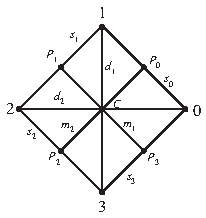
\includegraphics[width=0.282\linewidth,height=.8\textheight,keepaspectratio]{assets/p151_00.pdf}\end{center}
\begin{center}\small\textbf{14.10 Figure}\end{center}
\end{BookFloat}

We can think of the set

\begin{center}\begin{adjustbox}{max width=\linewidth}\BookInline{\displaystyle X= \{0,\allowbreak 1,\allowbreak 2,\allowbreak 3,\allowbreak s_{0},\allowbreak s_{1},\allowbreak s_{2},\allowbreak s_{3},\allowbreak m_{1},\allowbreak m_{2},\allowbreak d_{1},\allowbreak d_{2},\allowbreak C,\allowbreak P_{0},\allowbreak P_{1},\allowbreak P_{2},\allowbreak P_{3}\}}\end{adjustbox}\end{center}

\noindent as a \BookInline{D_{4}-}set in a natural way. Table 14.11 shows the action of \BookInline{D_{4}} on \BookInline{X.} Recall that \BookInline{\iota } is the identity\BookInline{,\allowbreak \rho ^{k}} is rotation by \BookInline{k\pi /2,\allowbreak } and \BookInline{\mu } is reflection across the line \BookInline{d_{2}.} We can see from the table that \BookInline{\mu \rho } is reflection across the line \BookInline{m_{1},\allowbreak \mu \rho ^{2}} is reflection across the line \BookInline{d_{1},\allowbreak } and \BookInline{\mu \rho ^{3}} is reflection across the line \BookInline{m_{2}.} It is worthwhile to spend a little time to understand how Table 14.11 was constructed before continuing\BookInline{.}\BookEnd{\blacktriangle}

\begin{BookFloat}{14_group_action_on_a_set-p151-4}
\BookStatement{\textbf{14.11 Table}}
\begin{center}\begin{adjustbox}{max width=\linewidth}\small\setlength{\tabcolsep}{3pt}
\begin{tabular}{c|ccccccccccccccccc}
\hline
 & \BookInline{0} & \BookInline{1} & \BookInline{2} & \BookInline{3} & \BookInline{s_0} & \BookInline{s_1} & \BookInline{s_2} & \BookInline{s_3} & \BookInline{m_1} & \BookInline{m_2} & \BookInline{d_1} & \BookInline{d_2} & \BookInline{C} & \BookInline{P_0} & \BookInline{P_1} & \BookInline{P_2} & \BookInline{P_3}\\\hline
\BookInline{\iota} & \BookInline{0} & \BookInline{1} & \BookInline{2} & \BookInline{3} & \BookInline{s_0} & \BookInline{s_1} & \BookInline{s_2} & \BookInline{s_3} & \BookInline{m_1} & \BookInline{m_2} & \BookInline{d_1} & \BookInline{d_2} & \BookInline{C} & \BookInline{P_0} & \BookInline{P_1} & \BookInline{P_2} & \BookInline{P_3}\\
\BookInline{\rho} & \BookInline{1} & \BookInline{2} & \BookInline{3} & \BookInline{0} & \BookInline{s_1} & \BookInline{s_2} & \BookInline{s_3} & \BookInline{s_0} & \BookInline{m_2} & \BookInline{m_1} & \BookInline{d_2} & \BookInline{d_1} & \BookInline{C} & \BookInline{P_1} & \BookInline{P_2} & \BookInline{P_3} & \BookInline{P_0}\\
\BookInline{\rho^2} & \BookInline{2} & \BookInline{3} & \BookInline{0} & \BookInline{1} & \BookInline{s_2} & \BookInline{s_3} & \BookInline{s_0} & \BookInline{s_1} & \BookInline{m_1} & \BookInline{m_2} & \BookInline{d_1} & \BookInline{d_2} & \BookInline{C} & \BookInline{P_2} & \BookInline{P_3} & \BookInline{P_0} & \BookInline{P_1}\\
\BookInline{\rho^3} & \BookInline{3} & \BookInline{0} & \BookInline{1} & \BookInline{2} & \BookInline{s_3} & \BookInline{s_0} & \BookInline{s_1} & \BookInline{s_2} & \BookInline{m_2} & \BookInline{m_1} & \BookInline{d_2} & \BookInline{d_1} & \BookInline{C} & \BookInline{P_3} & \BookInline{P_0} & \BookInline{P_1} & \BookInline{P_2}\\
\BookInline{\mu} & \BookInline{0} & \BookInline{3} & \BookInline{2} & \BookInline{1} & \BookInline{s_3} & \BookInline{s_2} & \BookInline{s_1} & \BookInline{s_0} & \BookInline{m_1} & \BookInline{m_2} & \BookInline{d_2} & \BookInline{d_1} & \BookInline{C} & \BookInline{P_3} & \BookInline{P_2} & \BookInline{P_1} & \BookInline{P_0}\\
\BookInline{\mu\rho} & \BookInline{3} & \BookInline{2} & \BookInline{1} & \BookInline{0} & \BookInline{s_2} & \BookInline{s_1} & \BookInline{s_0} & \BookInline{s_3} & \BookInline{m_2} & \BookInline{m_1} & \BookInline{d_1} & \BookInline{d_2} & \BookInline{C} & \BookInline{P_2} & \BookInline{P_1} & \BookInline{P_0} & \BookInline{P_3}\\
\BookInline{\mu\rho^2} & \BookInline{2} & \BookInline{1} & \BookInline{0} & \BookInline{3} & \BookInline{s_1} & \BookInline{s_0} & \BookInline{s_3} & \BookInline{s_2} & \BookInline{m_1} & \BookInline{m_2} & \BookInline{d_2} & \BookInline{d_1} & \BookInline{C} & \BookInline{P_1} & \BookInline{P_0} & \BookInline{P_3} & \BookInline{P_2}\\
\BookInline{\mu\rho^3} & \BookInline{1} & \BookInline{0} & \BookInline{3} & \BookInline{2} & \BookInline{s_0} & \BookInline{s_3} & \BookInline{s_2} & \BookInline{s_1} & \BookInline{m_2} & \BookInline{m_1} & \BookInline{d_1} & \BookInline{d_2} & \BookInline{C} & \BookInline{P_0} & \BookInline{P_3} & \BookInline{P_2} & \BookInline{P_1}\\
\hline\end{tabular}\end{adjustbox}\end{center}
\end{BookFloat}

\BookTextHeading{\textbf{Isotropy Subgroups}  }

\noindent Let \BookInline{X} be a \BookInline{G-}set. Let \BookInline{x\in X} and \BookInline{g\in G.} It will be important to know when \BookInline{gx= x.} We let

\begin{center}\begin{adjustbox}{max width=\linewidth}\BookInline{\displaystyle X_{g}= \{x\in X\mid gx= x\}\;\text{and}\;G_{x}= \{g\in G\mid gx= x\}.}\end{adjustbox}\end{center}

\BookLabel{14.12 Example} For the \BookInline{D_{4}-}set \BookInline{X} in Example 14.9, we have

\begin{center}\begin{adjustbox}{max width=\linewidth}\BookInline{\displaystyle X_{\iota }= X,\allowbreak }\end{adjustbox}\end{center}

\begin{center}\begin{adjustbox}{max width=\linewidth}\BookInline{\displaystyle X_{\rho }= \{C\},\allowbreak }\end{adjustbox}\end{center}

\begin{center}\begin{adjustbox}{max width=\linewidth}\BookInline{\displaystyle X_{\mu }= \{0,\allowbreak 2,\allowbreak d_{1},\allowbreak d_{2},\allowbreak C\}.}\end{adjustbox}\end{center}

Also, using the same \BookInline{D_{4}} action on \BookInline{X,\allowbreak }

\begin{center}\begin{adjustbox}{max width=\linewidth}\BookInline{\displaystyle G_{0}= \{\iota ,\allowbreak \mu \},\allowbreak }\end{adjustbox}\end{center}

\begin{center}\begin{adjustbox}{max width=\linewidth}\BookInline{\displaystyle G_{s_{2}}= \{\iota ,\allowbreak \mu \rho ^{3}\},\allowbreak }\end{adjustbox}\end{center}

\begin{center}\begin{adjustbox}{max width=\linewidth}\BookInline{\displaystyle G_{d_{1}}= \{\iota ,\allowbreak \rho ^{2},\allowbreak \mu ,\allowbreak \mu \rho ^{2}\}.}\end{adjustbox}\end{center}

We leave the computations of the other sets of the form \BookInline{X_{\sigma }} and \BookInline{G_{x}} to Exercises 1 and \BookInline{2.}\BookEnd{\blacktriangle}

Note that the subsets \BookInline{G_{x}} given in the preceding example were, in each case, subgroups of \BookInline{G.} This is true in general.

\end{BookBody}

% Source PDF page 152; original printed page 135
\BookSource{152}{135}
\BookNarrativetrue

\begin{BookBody}

\BookLabel{14.13 Theorem} Let \BookInline{X} be a \BookInline{G-}set. Then \BookInline{G_{x}} is a subgroup of \BookInline{G} for each \BookInline{x\in X.}

\BookLabel{\textit{Proof}} Let \BookInline{x\in X} and let \BookInline{g_{1},\allowbreak g_{2}\in G_{x}.} Then \BookInline{g_{1}x= x} and \BookInline{g_{2}x= x.} Consequently\BookInline{,\allowbreak (g_{1}g_{2})x= } \BookInline{g_{1}(g_{2}x)= g_{1}x= x,\allowbreak } so \BookInline{g_{1}g_{2}\in G_{x},\allowbreak } and \BookInline{G_{x}} is closed under the induced operation of \BookInline{G.} Of course,\textit{ ex} \BookInline{= x,\allowbreak } so \BookInline{e\in G_{x}.} If \BookInline{g\in G_{x},\allowbreak } then \BookInline{gx= x,\allowbreak } so \BookInline{x= } \textit{ex} \BookInline{= (g^{- 1}g)x= g^{- 1}(gx)= } \BookInline{g^{- 1}x,\allowbreak } and consequently \BookInline{g^{- 1}\in G_{x}.} Thus \BookInline{G_{x}} is a subgroup of \BookInline{G.}\BookEnd{\blacklozenge}

\BookLabel{14.14 Definition} Let \BookInline{X} be a \BookInline{G-}set and let \BookInline{x\in X.} The subgroup \BookInline{G_{x}} is the\textbf{ isotropy subgroup of} \BookInline{x.}\BookEnd{\blacksquare}

\BookTextHeading{\textbf{Orbits}}

\noindent For the \BookInline{D_{4}-}set \BookInline{X} of Example 14.9 with action table in Table 14.11, the elements in the subset \BookInline{\{0,\allowbreak 1,\allowbreak 2,\allowbreak 3\}} are carried into elements of this same subset under action by \BookInline{D_{4}.} Furthermore, each of the elements 0, 1, 2, and 3 is carried into all the other elements of the subset by the various elements of \BookInline{D_{4}.} We proceed to show that every \BookInline{G-}set \BookInline{X} can be partitioned into subsets of this type.

\BookLabel{14.15 Theorem} Let \BookInline{X} be a \BookInline{G-}set. For \BookInline{x_{1},\allowbreak x_{2}\in X,\allowbreak } let \BookInline{x_{1}\sim x_{2}} if and only if there exists \BookInline{g\in G} such that \BookInline{gx_{1}= x_{2}.} Then \BookInline{\sim } is an equivalence relation on \BookInline{X.}

\BookLabel{\textit{Proof}} For each \BookInline{x\in X,\allowbreak } we have\textit{ ex} \BookInline{= x,\allowbreak } so \BookInline{x\sim x} and \BookInline{\sim } is reflexive.

Suppose \BookInline{x_{1}\sim x_{2},\allowbreak } so \BookInline{gx_{1}= x_{2}} for some \BookInline{g\in G.} Then \BookInline{g^{- 1}x_{2}= g^{- 1}(gx_{1})= } \BookInline{(g^{- 1}g)x_{1}= ex_{1}= x_{1},\allowbreak } so \BookInline{x_{2}\sim x_{1},\allowbreak } and \BookInline{\sim } is symmetric.

Finally, if \BookInline{x_{1}\sim x_{2}} and \BookInline{x_{2}\sim x_{3},\allowbreak } then \BookInline{g_{1}x_{1}= x_{2}} and \BookInline{g_{2}x_{2}= x_{3}} for some \BookInline{g_{1},\allowbreak g_{2}\in G.} Then \BookInline{(g_{2}g_{1})x_{1}= g_{2}(g_{1}x_{1})= g_{2}x_{2}= x_{3},\allowbreak } so \BookInline{x_{1}\sim x_{3}} and \BookInline{\sim } is transitive\BookInline{.}\BookEnd{\blacklozenge}

\BookLabel{14.16 Definition} Let \BookInline{X} be a \BookInline{G-}set. Each cell in the partition of the equivalence relation described in Theorem 14.15 is an\textbf{ orbit in} \BookInline{X} \textbf{under} \BookInline{G.} If \BookInline{x\in X,\allowbreak } the cell containing \BookInline{x} is the\textbf{ orbit} \textbf{of} \BookInline{x.} We let this cell be \BookInline{Gx.}\BookEnd{\blacksquare}

The relationship between the orbits in \BookInline{X} and the group structure of \BookInline{G} lies at the heart of many applications. The following theorem gives this relationship. Recall that for a set \BookInline{X,\allowbreak } we use \BookInline{|X|} for the number of elements in \BookInline{X,\allowbreak } and \BookInline{(G:H)} is the index of a subgroup \BookInline{H} in a group \BookInline{G.}

\BookLabel{14.17 Theorem} Let \BookInline{X} be a \BookInline{G-}set and let \BookInline{x\in X.} Then \BookInline{|Gx|= (G:G_{x}).} If \BookInline{|G|} is finite, then \BookInline{|Gx|} is a divisor of \BookInline{|G|.}

\BookLabel{\textit{Proof}} We define a one-to-one map \BookInline{\psi } from \BookInline{Gx} onto the collection of left cosets of \BookInline{G_{x}} in \BookInline{G.} Let \BookInline{x_{1}\in Gx.} Then there exists \BookInline{g_{1}\in G} such that \BookInline{g_{1}x= x_{1}.} We define \BookInline{\psi (x_{1})} to be the left coset \BookInline{g_{1}G_{x}} of \BookInline{G_{x}.} We must show that this map \BookInline{\psi } is well defined, independent of the choice of \BookInline{g_{1}\in G} such that \BookInline{g_{1}x= x_{1}.} Suppose also that \BookInline{g_{1}^{\prime }x= x_{1}.} Then\BookInline{,\allowbreak g_{1}x= g_{1}^{\prime }x,\allowbreak } so \BookInline{g_{1}^{- 1}(g_{1}x)= g_{1}^{- 1}(g_{1}^{\prime }x),\allowbreak } from which we deduce \BookInline{x= (g_{1}^{- 1}g_{1}^{\prime })x.} Therefore \BookInline{g_{1}^{- 1}g_{1}^{\prime }\in G_{x},\allowbreak } so \BookInline{g_{1}^{\prime }\in g_{1}G_{x},\allowbreak } and \BookInline{g_{1}G_{x}= g_{1}^{\prime }G_{x}.} Thus the map \BookInline{\psi } is well defined.

To show the map \BookInline{\psi } is one-to-one, suppose \BookInline{x_{1},\allowbreak x_{2}\in Gx,\allowbreak } and \BookInline{\psi (x_{1})= \psi (x_{2}).} Then there exist \BookInline{g_{1},\allowbreak g_{2}\in G} such that \BookInline{x_{1}= g_{1}x,\allowbreak x_{2}= g_{2}x,\allowbreak } and \BookInline{g_{2}\in g_{1}G_{x}.} Then \BookInline{g_{2}= g_{1}g} for some \BookInline{g\in G_{x},\allowbreak } so \BookInline{x_{2}= g_{2}x= g_{1}(gx)= g_{1}x= x_{1}.} Thus \BookInline{\psi } is one-to-one.

Finally, we show that each left coset of \BookInline{G_{x}} in \BookInline{G} is of the form \BookInline{\psi (x_{1})} for some \BookInline{x_{1}\in Gx.} Let \BookInline{g_{1}G_{x}} be a left coset. Then if \BookInline{g_{1}x= x_{1},\allowbreak } we have \BookInline{g_{1}G_{x}= \psi (x_{1}).} Thus \BookInline{\psi } maps \BookInline{Gx} one-to-one onto the collection of left cosets so \BookInline{|Gx|= (G:G_{x}).}

If \BookInline{|G|} is finite, then the equation \BookInline{|G|= |G_{x}|(G:G_{x})} shows that \BookInline{|Gx|= (G:G_{x})} is a divisor of \BookInline{|G|.}\BookEnd{\blacklozenge}

\end{BookBody}

% Source PDF page 153; original printed page 136
\BookSource{153}{136}
\BookNarrativetrue

\begin{BookBody}

\BookLabel{14.18 Example} Let \BookInline{X} be the \BookInline{D_{4}-}set in Example 14.9, with action table given by Table 14.11. With \BookInline{G= D_{4},\allowbreak } we have \BookInline{G_{0}= \{\iota,\allowbreak \mu \}.} Since \BookInline{|G|= 8,\allowbreak } we have \BookInline{|G0|= (G:G_{0})= 4.} From Table 14.11, we see that \BookInline{G0= \{0,\allowbreak 1,\allowbreak 2,\allowbreak 3\},\allowbreak } which indeed has four elements\BookInline{.}\BookEnd{\blacktriangle}

We should remember not only the cardinality equation in Theorem 14.17 but also that the\textit{ elements of} \BookInline{G} \textit{carrying} \BookInline{x} \textit{into} \BookInline{g_{1}x} \textit{are precisely the elements of the left coset} \BookInline{g_{1}G_{x}.} Namely, if \BookInline{g\in G_{x},\allowbreak } then \BookInline{(g_{1}g)x= g_{1}(gx)= g_{1}x.} On the other hand, if \BookInline{g_{2}x= g_{1}x,\allowbreak } then \BookInline{g_{1}^{- 1}(g_{2}x)= x} so \BookInline{(g_{1}^{- 1}g_{2})x= x.} Thus \BookInline{g_{1}^{- 1}g_{2}\in G_{x}} so \BookInline{g_{2}\in g_{1}G_{x}.}

\BookTextHeading{\textbf{Applications of} \textit{\textbf{G}}\textbf{-Sets to Finite Groups}    }

\noindent Theorem 14.17 is a very useful theorem in the study of finite groups. Suppose that \BookInline{X} is a \BookInline{G-}set for a finite group \BookInline{G} and we pick out one element from each orbit of \BookInline{X} to make the set \BookInline{S= \{x_{1},\allowbreak x_{2},\allowbreak...,\allowbreak x_{r}\}} where we indexed the elements of \BookInline{X} so that if \BookInline{i\leq j,\allowbreak } then \BookInline{|Gx_{i}|\geq |Gx_{j}|.} That is, we arrange by orbit size, largest first and smallest last. Every element in \BookInline{X} is in precisely one orbit, so

\begin{center}\begin{adjustbox}{max width=\linewidth}\BookInline{\displaystyle |X|= \sum _{i= 1}^{r}|Gx_{i}|.(1)}\end{adjustbox}\end{center}

\noindent We let \BookInline{X_{G}= \{x\in X\mid gx= x} for all \BookInline{g\in G\}.} That is\BookInline{,\allowbreak X_{G}} is the set of all elements of \BookInline{X} whose orbit size is 1. So by equation (1),

\begin{center}\begin{adjustbox}{max width=\linewidth}\BookInline{\displaystyle |X|= |X_{G}|+ \sum _{i= 1}^{s}|Gx_{i}|(2)}\end{adjustbox}\end{center}

\noindent where we simply place all the orbits with one element into \BookInline{X_{G}} and we are left with \BookInline{s} orbits each containing at least two elements. Although Equation (2) is simply saying that if you add up the sizes of all the orbits you account for all the elements of \BookInline{X,\allowbreak } when coupled with Theorem 14.17, it gives some very interesting results. We give a few in the remainder of this section. In Section 17 we will use Equation 2 extensively to prove the Sylow Theorems.

For the remainder of this section,\textit{ we assume that} \BookInline{p} \textit{is} \BookInline{a} \textit{prime number}.

\BookLabel{14.19 Theorem} Let \BookInline{G} be a group with \BookInline{p^{n}} elements. If \BookInline{X} is a \BookInline{G-}set, then \BookInline{|X|\equiv |X_{G}|} mod \BookInline{p.}

\BookLabel{\textit{Proof}} Using Equation 2,

\begin{center}\begin{adjustbox}{max width=\linewidth}\BookInline{\displaystyle |X|= |X_{G}|+ \sum _{i= 1}^{s}|Gx_{i}|.}\end{adjustbox}\end{center}

\noindent Since for each \BookInline{i\leq s,\allowbreak |Gx_{i}|\geq 2} and \BookInline{|Gx_{i}|= (G:G_{x_{i}})} is a divisor of \BookInline{|G|= p^{n},\allowbreak } by Theorem \BookInline{14.17p} divides each term in the sum \BookInline{\sum _{i= 1}^{s}|Gx_{i}|.} Thus \BookInline{|X|\equiv |X_{G}|} mod \BookInline{p.}\BookEnd{\blacklozenge}

\noindent Knowing that \BookInline{k} divides the order of a group is not sufficient information to assume that the group has a subgroup of order \BookInline{k.} For example, we saw that \BookInline{A_{4}} has no subgroup of order 6 and that in general\BookInline{,\allowbreak A_{n}} has no subgroup of index 2 if \BookInline{n\geq 4.} On the positive side, in Exercise 29 in Section 2, you were asked to show that if a group has an even number of elements, then it has an element of order two. Theorem 14.20 generalizes this result to show that if a prime number \BookInline{p} divides the order of a group, then the group has an element of order \BookInline{p.} The proof of this theorem relies on Theorem 14.19.

\BookLabel{14.20 Theorem} \textbf{(Cauchy’s Theorem)} Let \BookInline{G} be a group such that \BookInline{p} divides the order of \BookInline{G.} Then \BookInline{G} has an element of order \BookInline{p} and therefore a subgroup of order \BookInline{p.}

\end{BookBody}

% Source PDF page 154; original printed page 137
\BookSource{154}{137}
\BookNarrativetrue

\begin{BookBody}

\BookLabel{\textit{Proof}} We let

\begin{center}\begin{adjustbox}{max width=\linewidth}\BookInline{\displaystyle X= \{(g_{0},\allowbreak g_{1},\allowbreak g_{2},\allowbreak ...,\allowbreak g_{p- 1})\mid g_{0},\allowbreak g_{1},\allowbreak ...,\allowbreak g_{p- 1}\in G\;\text{and}\;g_{0}g_{1}g_{2}...g_{p- 1}= e\}.}\end{adjustbox}\end{center}

\noindent That is\BookInline{,\allowbreak X} is the set of all \BookInline{p-}tuples with entries in \BookInline{G} so that when the entries are multiplied together (in order) their product is the identity \BookInline{e.} Since the product is \BookInline{e,\allowbreak g_{0}= } \BookInline{(g_{1}g_{2}...g_{p- 1})^{- 1}} and given any \BookInline{g_{1},\allowbreak g_{2},\allowbreak...,\allowbreak g_{p- 1}\in G,\allowbreak } by picking \BookInline{g_{0}= (g_{1}g_{2}...g_{p- 1})^{- 1}} we have an element in \BookInline{X.} Thus \BookInline{|X|= |G|^{p- 1}} and in particular\BookInline{,\allowbreak p} divides the order of \BookInline{X} since \BookInline{p} divides the order of \BookInline{G.}

\begingroup\sloppy Suppose that \BookInline{(g_{0},\allowbreak g_{1},\allowbreak g_{2},\allowbreak...,\allowbreak g_{p- 1})\in X.} Since \BookInline{g_{0}= (g_{1}g_{2}...g_{p- 1})^{- 1},\allowbreak } it follows that \BookInline{(g_{1},\allowbreak g_{2},\allowbreak...g_{p- 1},\allowbreak g_{0})} is in \BookInline{X.} Repeating this process, noting that \BookInline{g_{1}= (g_{2}g_{3}...g_{p- 1}g_{0})^{- 1}} we conclude that \BookInline{(g_{2},\allowbreak g_{3},\allowbreak g_{4},\allowbreak \cdots,\allowbreak g_{p- 1},\allowbreak g_{0},\allowbreak g_{1})\in X.} Continuing in this manner we have that for any \BookInline{k\in \mathbb{Z}_{p},\allowbreak }\par\endgroup

\begin{center}\begin{adjustbox}{max width=\linewidth}\BookInline{\displaystyle (g_{k},\allowbreak g_{k+ _{p}1},\allowbreak g_{k+ _{p}2},\allowbreak ...,\allowbreak g_{k+ _{p}(p- 1)})\in X.}\end{adjustbox}\end{center}

\noindent We check that this gives a group action of \BookInline{\mathbb{Z}_{p}} on \BookInline{X.} Let \BookInline{k\in \mathbb{Z}_{p}} and \BookInline{(g_{0},\allowbreak g_{1},\allowbreak g_{2},\allowbreak...,\allowbreak g_{p- 1})\in } \BookInline{X.} Then

\begin{center}\begin{adjustbox}{max width=\linewidth}\BookInline{\displaystyle k(g_{0},\allowbreak g_{1},\allowbreak g_{2},\allowbreak ...,\allowbreak g_{p- 1})= (g_{k},\allowbreak g_{k+ _{p}1},\allowbreak g_{k+ _{p}2},\allowbreak ...,\allowbreak g_{k+ _{p}(p- 1)})\in X.}\end{adjustbox}\end{center}

\noindent Since

\begin{center}\begin{adjustbox}{max width=\linewidth}\BookInline{\displaystyle 0(g_{0},\allowbreak g_{1},\allowbreak g_{2},\allowbreak ...,\allowbreak g_{p- 1})= (g_{0},\allowbreak g_{1},\allowbreak g_{2},\allowbreak ...,\allowbreak g_{p- 1})\;\text{and}\;}\end{adjustbox}\end{center}

\begin{center}\begin{adjustbox}{max width=\linewidth}\BookInline{\displaystyle \begin{aligned}k(l(g_{0},\allowbreak g_{1},\allowbreak g_{2},\allowbreak ...,\allowbreak g_{p- 1}))&= k(g_{l},\allowbreak g_{l+ _{p}1},\allowbreak g_{l+ _{p}2},\allowbreak ...,\allowbreak g_{l+ _{p}(p- 1)}) \\ &= (g_{k+ _{p}l},\allowbreak g_{k+ _{p}l+ _{p}1},\allowbreak ...,\allowbreak g_{k+ _{p}l+ _{p}(p- 1)}) \\ &= (k+ _{p}l)(g_{0},\allowbreak g_{1},\allowbreak g_{2},\allowbreak ...,\allowbreak g_{p- 1})\end{aligned}}\end{adjustbox}\end{center}

\noindent this is indeed a group action.

By Theorem 14. \BookInline{19,\allowbreak 0\equiv |X|\equiv |X_{\mathbb{Z}_{p}}|} mod \BookInline{p.} The \BookInline{p-}tuple \BookInline{(e,\allowbreak e,\allowbreak e,\allowbreak...,\allowbreak e)} is in \BookInline{X_{\mathbb{Z}_{p}}} because rearranging the entries does not change the \BookInline{p-}tuple. Since \BookInline{X_{\mathbb{Z}_{p}}} contains at least one element and \BookInline{p} divides \BookInline{|X_{\mathbb{Z}_{p}}|,\allowbreak X_{\mathbb{Z}_{p}}} must contain at least one element other than \BookInline{(e,\allowbreak e,\allowbreak e,\allowbreak...,\allowbreak e).} That element must have the form \BookInline{(a,\allowbreak a,\allowbreak a,\allowbreak...,\allowbreak a)} with \BookInline{a\neq e} and \BookInline{a^{p}= e.} So \BookInline{a} has order \BookInline{p} and the subgroup it generates is a subgroup of \BookInline{G} with order \BookInline{p.}\BookEnd{\blacklozenge}

\BookLabel{14.21 Definition} A \BookInline{p-}group is a group such that each element in the group has order a power of \BookInline{p.} A \BookInline{p-}subgroup of a group is a subgroup that is a \BookInline{p-}group\BookInline{.}\BookEnd{\blacksquare}

\BookLabel{14.22 Example} The group \BookInline{D_{16}} is a 2-group since the order of any element of \BookInline{D_{16}} divides \BookInline{|D_{16}|= 32.} \BookEnd{\blacktriangle}

\BookLabel{14.23 Example} Using the Fundamental Theorem of Finitely Generated Abelian Groups, a finite abelian group is a \BookInline{p-}group if and only if it is isomorphic to

\begin{center}\begin{adjustbox}{max width=\linewidth}\BookInline{\displaystyle \mathbb{Z}_{p^{1}}^{r}\times \mathbb{Z}_{p^{2}}^{r}\times \mathbb{Z}_{p^{3}}^{r}\times \cdots \times \mathbb{Z}_{p}rn.}\end{adjustbox}\end{center}

\noindent This is because if there were a factor of the form \BookInline{\mathbb{Z}_{q}s} where \BookInline{q\neq p} is a prime number and \BookInline{s\geq 1,\allowbreak } then there would be an element in \BookInline{G} with order \BookInline{q^{s}} which is not a power of \BookInline{p.}

In Exercise 30, you are asked to show that for \BookInline{G} a finite group\BookInline{,\allowbreak G} is a \BookInline{p-}group if and only if the order of \BookInline{G} is a power of \BookInline{p.}

The next theorem assures us that any finite \BookInline{p-}group has a nontrivial normal subgroup, namely the center of the group\BookInline{.}\BookEnd{\blacktriangle}

\BookLabel{14.24 Theorem} Let \BookInline{G} be a finite \BookInline{p-}group. Then the center of \BookInline{G,\allowbreak Z(G),\allowbreak } is not the trivial group.

\BookLabel{\textit{Proof}} We let \BookInline{X= G} and we make \BookInline{X} into a \BookInline{G-}set using conjugation. That is\BookInline{,\allowbreak \ast (g,\allowbreak a)= gag^{- 1}.} Equation 2 states that \BookInline{0\equiv |X|\equiv |X_{G}|} mod \BookInline{p.} For all \BookInline{g\in G,\allowbreak geg^{- 1}= e.} So \BookInline{X_{G}} has at 
% Source PDF page 155; original printed page 138
\BookSource{155}{138}
least one element, namely \BookInline{e.} Since the number of elements in \BookInline{X_{G}} must be at least \BookInline{p,\allowbreak } there is an element \BookInline{a\in X} such that \BookInline{a\neq e} and \BookInline{gag^{- 1}= a} for all \BookInline{g\in G.} Thus \BookInline{ga= ag} for all \BookInline{g\in G,\allowbreak } which says that \BookInline{a\in Z(G).} So \BookInline{Z(G)} is not the trivial subgroup\BookInline{.}\BookEnd{\blacklozenge}

\end{BookBody}

\BookNarrativetrue

\begin{BookBody}

\noindent When studying \BookInline{p-}groups, the fact that the center is nontrivial is often very helpful. We conclude this section with a theorem that illustrates the utility of Theorem 14.24.

\BookLabel{14.25 Theorem} Every group of order \BookInline{p^{2}} is abelian.

\BookLabel{\textit{Proof}} Let \BookInline{G} be a group of order \BookInline{p^{2}} with center \BookInline{Z(G).} By Theorem \BookInline{14.24,\allowbreak Z(G)} is not the trivial group so it is either all of \BookInline{G} or else it has order \BookInline{p.} We wish to show that \BookInline{Z(G)= G} using proof by contradiction. So we assume that \BookInline{Z(G)} has \BookInline{p} elements. Since \BookInline{Z(G)} is a normal subgroup of \BookInline{G,\allowbreak } we can form \BookInline{G/Z(G).} The group \BookInline{G/Z(G)} also has \BookInline{p} elements and so both \BookInline{Z(G)} and \BookInline{G/Z(G)} are cyclic. Let \BookInline{\langle a\rangle = Z(G)} and \BookInline{\langle bZ(G)\rangle = G/Z(G).} Let \BookInline{x,\allowbreak y\in G.} Then \BookInline{x= b^{i}a^{j}} and \BookInline{y= b^{r}a^{s}} for some integers \BookInline{i,\allowbreak j,\allowbreak r,\allowbreak s} since the cosets of \BookInline{Z(G)} partition \BookInline{G.} Then

\begin{center}\begin{adjustbox}{max width=\linewidth}\BookInline{\displaystyle xy= b^{i}a^{j}b^{r}a^{s}= b^{i}b^{r}a^{j}a^{s}}\end{adjustbox}\end{center}

\noindent since \BookInline{\langle a\rangle } is the center of \BookInline{G.} So

\begin{center}\begin{adjustbox}{max width=\linewidth}\BookInline{\displaystyle xy= b^{i+ r}a^{j+ s}= b^{r}b^{i}a^{s}a^{j}= b^{r}a^{s}b^{i}a^{j}= yx.}\end{adjustbox}\end{center}

\noindent Since every element in \BookInline{G} commutes with every other element\BookInline{,\allowbreak Z(G)= G,\allowbreak } which contradicts our assumption that the center has only \BookInline{p} elements. So the center of \BookInline{G} must be \BookInline{G,\allowbreak } which means that \BookInline{G} is abelian\BookInline{.}\BookEnd{\blacklozenge}

\BookLabel{14.26 Example} Since every group of order \BookInline{p^{2}} is abelian, the Fundamental Homomorphism Theorem says that every group with \BookInline{p^{2}} elements is isomorphic to either \BookInline{\mathbb{Z}_{p}2\;\text{or}\;\mathbb{Z}_{p}\times \mathbb{Z}_{p}.} The two groups of order 4 are \BookInline{\mathbb{Z}_{4}} and the Klein 4-group. The two groups of order 9 are \BookInline{\mathbb{Z}_{9}} and \BookInline{\mathbb{Z}_{3}\times \mathbb{Z}_{3}.}\BookEnd{\blacktriangle}

\end{BookBody}

\BookNarrativefalse

\begin{BookBody}

\BookExerciseTitle{14}

\BookTextHeading{\textbf{Computations}}

\noindent In Exercises 1 through 3, let

\begin{center}\begin{adjustbox}{max width=\linewidth}\BookInline{\displaystyle X= \{0,\allowbreak 1,\allowbreak 2,\allowbreak 3,\allowbreak s_{0},\allowbreak s_{1},\allowbreak s_{2},\allowbreak s_{3},\allowbreak m_{1},\allowbreak m_{2},\allowbreak d_{1},\allowbreak d_{2},\allowbreak C,\allowbreak P_{0},\allowbreak P_{1},\allowbreak P_{2},\allowbreak P_{3}\}}\end{adjustbox}\end{center}

\noindent be the \BookInline{D_{4}-}set of Example 14.9. Find the following, where \BookInline{G= D_{4}.}

\BookExercise{1.}{The fixed sets \BookInline{X_{\sigma }} for each \BookInline{\sigma \in D_{4}.}}

\BookExercise{2.}{The isotropy subgroups \BookInline{G_{x}} for each \BookInline{x\in X,\allowbreak } that is\BookInline{,\allowbreak G_{0},\allowbreak G_{1},\allowbreak \cdots,\allowbreak G_{P_{2}},\allowbreak G_{P_{3}}.}}

\BookExercise{3.}{The orbits in \BookInline{X} under \BookInline{D_{4}.}}

\BookExercise{4.}{Theorem 14.24 states that every \BookInline{p-}group has nontrivial center. Find the center of \BookInline{D_{8}.}}

\BookExercise{5.}{Find the center of \BookInline{D_{7}.}}

\BookExercise{6.}{Let \BookInline{G= X= S_{3}} and make \BookInline{X} a \BookInline{G-}set using conjugation. That is\BookInline{,\allowbreak \ast (\sigma,\allowbreak \tau )= \sigma \tau \sigma ^{- 1}.} Find all the orbits of \BookInline{X} using this action. (Write permutations in disjoint cycle notation.)}

\BookExercise{7.}{Let \BookInline{G= D_{4}} and \BookInline{X} be the set of all subgroups of \BookInline{D_{4}} with order two. The set \BookInline{X} is a \BookInline{G-}set using conjugation, \BookInline{\ast (\sigma,\allowbreak H)= \sigma H\sigma ^{- 1}.} Find all the orbits of this group action.}

\BookExercise{8.}{Let \BookInline{G= U= \{z\in \mathbb{C}\mid |z|= 1\}} be the circle group. Then \BookInline{X= \mathbb{C},\allowbreak } the set of complex numbers, is a \BookInline{G-}set with group action given by complex number multiplication. That is, if \BookInline{z\in U} and \BookInline{w\in \mathbb{C},\allowbreak \ast (z,\allowbreak w)= zw.} Find all the orbits of this action. Also, find \BookInline{X_{G}.}}

\end{BookBody}

% Source PDF page 156; original printed page 139
\BookSource{156}{139}
\BookNarrativefalse

\begin{BookBody}

\BookExercise{9.}{Let \BookInline{G} be a group of order 3 and suppose that \BookInline{|X|= 6.} For each possible action of \BookInline{G} on \BookInline{X,\allowbreak } give a list of the orbit sizes. List the orbit sizes from largest to smallest. (Recall that the orbits partition the set \BookInline{X.)}}

\BookExercise{10.}{Let \BookInline{G} be a group of order 9 and suppose that \BookInline{|X|= 10.} For each possible action of \BookInline{G} on \BookInline{X,\allowbreak } give a list of the orbit sizes. List the orbit sizes from largest to smallest.}

\BookExercise{11.}{Let \BookInline{G} be a group of order 8 and suppose that \BookInline{|X|= 10.} For each possible way to make \BookInline{X} a \BookInline{G-}set the orbits partition \BookInline{X.} For each possible action of \BookInline{G} on \BookInline{X,\allowbreak } give a list of the orbit sizes. List the orbit sizes from largest to smallest.}

\BookTextHeading{\textbf{Concepts}}

\noindent In Exercises 12 and 13, correct the definition of the italicized term without reference to the text, if correction is needed, so that it is in a form acceptable for publication.

\BookExercise{12.}{A group \BookInline{G} \textit{acts faithfully} on \BookInline{X} if and only if \BookInline{gx= x} implies that \BookInline{g= e.}}

\BookExercise{13.}{A group \BookInline{G} is\textit{ transitive} on a \BookInline{G-}set \BookInline{X} if and only if, for some \BookInline{g\in G,\allowbreak gx} can be every other \BookInline{x.}}

\BookExercise{14.}{Let \BookInline{X} be a \BookInline{G-}set and let \BookInline{S\subseteq X.} If \BookInline{Gs\subseteq S} for all \BookInline{s\in S,\allowbreak } then \BookInline{S} is a\textbf{ sub}\BookInline{-G-}\textbf{set.} Characterize a sub\BookInline{-G-}set of a \BookInline{G-}set \BookInline{X} in terms of orbits in \BookInline{X} under \BookInline{G.}}

\BookExercise{15.}{Characterize a transitive \BookInline{G-}set in terms of its orbits.}

\BookExercise{16.}{Determine whether each of the following is true or false.}

\BookExercise{a.}{Every \BookInline{G-}set is also a group.}

\BookExercise{b.}{Each element of a \BookInline{G-}set is fixed by the identity of \BookInline{G.}}

\BookExercise{c.}{If every element of a \BookInline{G-}set is fixed by the same element \BookInline{g} of \BookInline{G,\allowbreak } then \BookInline{g} must be the identity \BookInline{e.}}

\BookExercise{d.}{Let \BookInline{X} be a \BookInline{G-}set with \BookInline{x_{1},\allowbreak x_{2}\in X} and \BookInline{g\in G.} If \BookInline{gx_{1}= gx_{2},\allowbreak } then \BookInline{x_{1}= x_{2}.}}

\BookExercise{e.}{Let \BookInline{X} be a \BookInline{G-}set with \BookInline{x\in X} and \BookInline{g_{1},\allowbreak g_{2}\in G.} If \BookInline{g_{1}x= g_{2}x,\allowbreak } then \BookInline{g_{1}= g_{2}.}}

\BookExercise{f.}{Each orbit of a \BookInline{G-}set \BookInline{X} is a transitive sub\BookInline{-G-}set. (See Exercise 14.)}

\BookExercise{g.}{Let \BookInline{X} be a \BookInline{G-}set and let \BookInline{H\leq G.} Then \BookInline{X} can be regarded in a natural way as an \BookInline{H-}set.}

\BookExercise{h.}{With reference to (g), the orbits in \BookInline{X} under \BookInline{H} are the same as the orbits in \BookInline{X} under \BookInline{G.}}

\BookExercise{i.}{If \BookInline{X} is a \BookInline{G-}set, then each element of \BookInline{G} acts as a permutation of \BookInline{X.}}

\BookExercise{j.}{Let \BookInline{X} be a \BookInline{G-}set and let \BookInline{x\in X.} If \BookInline{G} is finite, then \BookInline{|G|= |Gx|\cdot |G_{x}|.}}

\BookExercise{17.}{Let \BookInline{X} and \BookInline{Y} be \BookInline{G-}sets with the\textit{ same} group \BookInline{G.} An\textbf{ isomorphism} between \BookInline{G-}sets \BookInline{X} and \BookInline{Y} is a map \BookInline{\phi:X\to Y} that is one-to-one, onto \BookInline{Y,\allowbreak } and satisfies \BookInline{g\phi (x)= \phi (gx)} for all \BookInline{x\in X} and \BookInline{g\in G.} Two \BookInline{G-}sets are\textbf{ isomorphic} if such an isomorphism between them exists. Let \BookInline{X} be the \BookInline{D_{4}-}set of Example 14.9.}

\BookExercise{a.}{Find two distinct orbits of \BookInline{X} that are isomorphic sub\BookInline{-D_{4}-}sets. (See Exercise 14.)}

\BookExercise{b.}{Show that the orbits \BookInline{\{0,\allowbreak 1,\allowbreak 2,\allowbreak 3\}} and \BookInline{\{s_{0},\allowbreak s_{1},\allowbreak s_{2},\allowbreak s_{3}\}} are not isomorphic sub\BookInline{-D_{4}-}sets. [\textit{Hint:} Find an element of \BookInline{G} that acts in an essentially different fashion on the two orbits.]}

\BookExercise{c.}{Are the orbits you gave for your answer to part (a) the only two different isomorphic sub\BookInline{-D_{4}-}sets of \BookInline{X}?}

\BookExercise{18.}{Let \BookInline{X} be the \BookInline{D_{4}-}set in Example 14.9.}

\BookExercise{a.}{Does \BookInline{D_{4}} act faithfully on \BookInline{X}?}

\BookExercise{b.}{Find all orbits in \BookInline{X} on which \BookInline{D_{4}} acts faithfully as a sub\BookInline{-D_{4}-}set. (See Exercise 14.)}

\BookTextHeading{\textbf{Theory}}

\BookExercise{19.}{Let \BookInline{X} be a \BookInline{G-}set. Show that \BookInline{G} acts faithfully on \BookInline{X} if and only if no two distinct elements of \BookInline{G} have the same action on each element of \BookInline{X.}}

\BookExercise{20.}{Let \BookInline{X} be a \BookInline{G-}set and let \BookInline{Y\subseteq X.} Let \BookInline{G_{Y}= \{g\in G\mid gy= y} for all \BookInline{y\in Y\}.} Show \BookInline{G_{Y}} is a subgroup of \BookInline{G,\allowbreak } generalizing Theorem 14.13.}

\BookExercise{21.}{Let \BookInline{G} be the additive group of real numbers. Let the action of \BookInline{\theta \in G} on the real plane \BookInline{\mathbb{R}^{2}} be given by rotating the plane counterclockwise about the origin through \BookInline{\theta } radians. Let \BookInline{P} be a point other than the origin in the plane.}

\BookExercise{a.}{Show \BookInline{\mathbb{R}^{2}} is a \BookInline{G-}set.}

\BookExercise{b.}{Describe geometrically the orbit containing \BookInline{P.}}

\BookExercise{c.}{Find the group \BookInline{G_{P}.}}

\end{BookBody}

% Continuation on source PDF page 157, preceding Section 15
\BookNarrativefalse

\begin{BookBody}

\noindent Exercises 22 through 25 show how all possible \BookInline{G-}sets, up to isomorphism (see Exercise 17), can be formed from the group \BookInline{G.}

\BookExercise{22.}{Let \BookInline{\{X_{i}\mid i\in I\}} be a disjoint collection of sets, so \BookInline{X_{i}\cap X_{j}= \emptyset } for \BookInline{i\neq j.} Let each \BookInline{X_{i}} be a \BookInline{G-}set for the same group \BookInline{G.}}

\BookExercise{a.}{Show that \BookInline{\bigcup _ { i \in I } X _ { i }} can be viewed in a natural way as a \BookInline{G-}set, the\textbf{ union} of the \BookInline{G-}sets \BookInline{X_{i}.}}

\BookExercise{b.}{Show that every \BookInline{G-}set \BookInline{X} is the union of its orbits.}

\BookExercise{23.}{Let \BookInline{X} be a transitive \BookInline{G-}set, and let \BookInline{x_{0}\in X.} Show that \BookInline{X} is isomorphic (see Exercise 17) to the \BookInline{G-}set \BookInline{L} of all left cosets of \BookInline{G_{x_{0}},\allowbreak } described in Example 14.8. [\textit{Hint:} For \BookInline{x\in X,\allowbreak } suppose \BookInline{x= gx_{0},\allowbreak } and define \BookInline{\phi:X\to L} by \BookInline{\phi (x)= gG_{x_{0}}.} Be sure to show \BookInline{\phi } is well defined!]}

\BookExercise{24.}{Let \BookInline{X_{i}} for \BookInline{i\in I} be \BookInline{G-}sets for the same group \BookInline{G,\allowbreak } and suppose the sets \BookInline{X_{i}} are not necessarily disjoint. Let \BookInline{X_{i}^{\prime }= \{(x,\allowbreak i)\mid x\in X_{i}\}} for each \BookInline{i\in I.} Then the sets \BookInline{X_{i}^{\prime }} are disjoint, and each can still be regarded as a \BookInline{G-}set in an obvious way. (The ele\BookInline{\cup }ments of \BookInline{X_{i}} have simply been tagged by \BookInline{i} to distinguish them from the elements of \BookInline{X_{j}} for \BookInline{i\neq j.)} The \BookInline{G-}set \BookInline{i\in IXi\prime } is the\textbf{ disjoint union} of the \BookInline{G-}sets \BookInline{X_{i}.} Using Exercises 22 and 23, show that every \BookInline{G-}set is isomorphic to a disjoint union of left coset \BookInline{G-}sets, as described in Example 14.12.}

\BookExercise{25.}{The preceding exercises show that every \BookInline{G-}set \BookInline{X} is isomorphic to a disjoint union of left coset \BookInline{G-}sets. The question then arises whether left coset \BookInline{G-}sets of distinct subgroups \BookInline{H} and \BookInline{K} of \BookInline{G} can themselves be isomorphic. Note that the map defined in the hint of Exercise 23 depends on the choice of \BookInline{x_{0}} as “base point.” If \BookInline{x_{0}} is replaced by \BookInline{g_{0}x_{0}} and if \BookInline{G _ { x _ { 0 } } \neq G _ { g _ { 0 } x _ { 0 } }.} then the collections \BookInline{L_{H}} of left cosets of \BookInline{H= G_{x_{0}}} and \BookInline{L_{K}} of left cosets of \BookInline{K= G_{g_{0}x_{0}}} form distinct \BookInline{G-}sets that must be isomorphic, since both \BookInline{L_{H}} and \BookInline{L_{K}} are isomorphic to \BookInline{X.}}

\BookExercise{a.}{Let \BookInline{X} be a transitive \BookInline{G-}set and let \BookInline{x_{0}\in X} and \BookInline{g_{0}\in G.} If \BookInline{H= G_{x_{0}},\allowbreak } describe \BookInline{K= G_{g_{0}x_{0}}} in terms of \BookInline{H} and \BookInline{g_{0}.}}

\BookExercise{b.}{Based on part (a), conjecture conditions on subgroups \BookInline{H} and \BookInline{K} of \BookInline{G} such that the left coset \BookInline{G-}sets of \BookInline{H} and \BookInline{K} are isomorphic.}

\BookExercise{c.}{Prove your conjecture in part (b).}

\BookExercise{26.}{Up to isomorphism, how many transitive \BookInline{\mathbb{Z}_{4}-}sets \BookInline{X} are there? (Use the preceding exercises.) Give an example of each isomorphism type, listing an action table of each as in Table 14.11. Take lowercase names \BookInline{a,\allowbreak b,\allowbreak c,\allowbreak } and so on for the elements in the set \BookInline{X.}}

\BookExercise{27.}{Repeat Exercise 26 for the group \BookInline{\mathbb{Z}_{6}.}}

\BookExercise{28.}{Repeat Exercise 26 for the group \BookInline{S_{3}.} List the elements of \BookInline{S_{3}} in the order \BookInline{\iota,\allowbreak (1,\allowbreak 2,\allowbreak 3),\allowbreak (1,\allowbreak 3,\allowbreak 2),\allowbreak (2,\allowbreak 3),\allowbreak (1,\allowbreak 3),\allowbreak } (1, 2).}

\BookExercise{29.}{Prove that if \BookInline{G} is a group of order \BookInline{p^{3},\allowbreak } where \BookInline{p} is a prime number, then \BookInline{|Z(G)|} is either \BookInline{p} or \BookInline{p^{3}.} Give an example where \BookInline{|Z(G)|= p} and an example where \BookInline{|Z(G)|= p^{3}.}}

\BookExercise{30.}{Let \BookInline{p} be a prime number. Prove that a finite group \BookInline{G} is a \BookInline{p-}group if and only if \BookInline{|G|= p^{n}} for some integer \BookInline{n\geq 0.}}

\BookExercise{31.}{Let \BookInline{G} be a group that acts on \BookInline{X= \{H\mid H\leq G\}} by conjugation. That is\BookInline{,\allowbreak g\ast H= gHg^{- 1}.} State and prove an equivalent condition for a subgroup \BookInline{H\leq G} to be a normal subgroup of \BookInline{G} in terms of}

\BookExercise{a.}{\textbf{a}\BookInline{.G_{H},\allowbreak } the isotropy subgroup of \BookInline{H.}}

\BookExercise{b.}{\textbf{b}\BookInline{.GH,\allowbreak } the orbit of \BookInline{H.}}

\end{BookBody}
\ifdefined\BookMaster\let\BookFinish\relax\else\def\BookFinish{\end{document}}\fi\BookFinish
